\documentclass[10pt,twocolumn,letterpaper]{article}

\usepackage[margin=0.72in,top=0.85in,bottom=0.85in]{geometry}
\usepackage{amsmath,amssymb,amsfonts}
\usepackage{graphicx}
\usepackage{booktabs}
\usepackage{microtype}
\usepackage{authblk}
\usepackage{xcolor}
\usepackage{caption}
\usepackage{float}
\usepackage{tabularx}
\usepackage{cite}
\usepackage[colorlinks=true,linkcolor=blue!70!black,citecolor=blue!70!black,urlcolor=blue!70!black]{hyperref}

% Typography & Header settings
\setlength{\columnsep}{0.25in}
\captionsetup{font=small,labelfont=bf}

\title{\textbf{\Large BioTransfer: Grounding Perturbation Biology in Multimodal Protein Language Priors and Cross-Lineage Screen Translation}}

\author[1,2,*]{\textbf{Md. Jubayer Hossain}}

\affil[1]{\small Center for Health Innovation, Research, Action, and Learning - Bangladesh (CHIRAL-BD), Dhaka, Bangladesh}
\affil[2]{\small DeepBio, Dhaka, Bangladesh}
\affil[*]{\small Corresponding author: \texttt{jubayer@chiralbd.org}}

\date{\small \today}

\begin{document}

\maketitle

\begin{abstract}
Predicting high-dimensional single-cell transcriptional responses to genetic perturbations is central to functional genomics and targeted therapeutic design. However, existing perturbation response models suffer from two critical architectural bottlenecks: (1) representations of genetic targets rely on discrete categorical tokens that cannot generalize out-of-distribution (OOD) to unseen genes, and (2) single-cell CRISPR screens are lineage-locked, failing to translate from cost-effective suspension cancer models (e.g., K562) into adherent, diploid human tissues (e.g., RPE1). Here, we introduce \textbf{BioTransfer}, a biologically grounded deep learning framework that resolves both bottlenecks. BioTransfer grounds genetic targets in continuous, evolutionary-scale protein language model embeddings (ESM-2) and conditions regulatory shifts on the recipient cell's basal state via Feature-wise Linear Modulation (FiLM). Furthermore, we establish \textbf{BioTransferTranslator}, a cross-lineage neural translation architecture that maps perturbation responses across cell lineages with learned protein-gated residual corrections. Evaluated across 2,055 aligned perturbations in the genome-scale Replogle 2022 benchmark, BioTransferTranslator achieves a \textbf{69.8\% error reduction} over empirical baselines on 308 dual zero-shot hold-out genes (Top-20 DE MSE drops from 0.3817 to 0.1152; Pearson $\rho$ jumps from 0.8613 to 0.9426). On combinatorial perturbations in Norman 2019, ESM-2 embedding arithmetic captures non-linear epistasis, achieving a \textbf{67.5\% error reduction} over literature mean shift baselines ($\rho = 0.9556$ vs $0.8788$). Systematic dissection reveals that while core proteostasis machinery is highly transferable across cell types ($\rho \approx 0.39$), cytoskeletal and mitochondrial networks exhibit pronounced lineage divergence ($\rho \approx 0.08$). BioTransfer establishes a generalizable, computationally portable paradigm for virtual screening across human cell lineages.
\end{abstract}

\section{Introduction}
Pooled single-cell CRISPR perturbation screening (Perturb-seq) enables the direct observation of transcriptomic consequences following targeted genetic disruptions at single-cell resolution \cite{dixit2016perturb, adamson2016multiplexed, norman2019exploring, replogle2022mapping}. While these screens provide unprecedented genotype-phenotype maps, the astronomical combinatorial space of human genes ($>20,000$ single knockouts and $>2 \times 10^8$ pairwise combinations) renders experimental profiling in every physiological context intractable. Consequently, machine learning architectures designed to predict transcriptional outcomes in silico have emerged as an active frontier \cite{roohani2023predicting, lotfollahi2019scgen, lotfollahi2023biologically}.

Despite significant architectural complexity, recent landmark benchmarks by Ahlmann-Eltze and Huber \cite{ahlmann2025benchmarking} revealed a cautionary reality: on rigorous out-of-distribution (OOD) unseen gene evaluations, state-of-the-art deep neural networks often fail to outperform simple empirical baselines, such as the mean shift of training perturbations. We identify two core conceptual flaws underlying this failure:
\begin{enumerate}
    \item \textbf{Tokenization of Biology:} Existing architectures (such as GEARS \cite{roohani2023predicting} and CPA \cite{lotfollahi2023biologically}) treat perturbed genes as arbitrary categorical IDs or lookup tokens. When a test gene was never observed during training, the network has no biological prior to infer its downstream functional impact.
    \item \textbf{The Lineage Barrier:} Genome-wide CRISPR screens are overwhelmingly conducted in suspension cancer cell lines (such as K562 chronic myelogenous leukemia) due to superior growth kinetics and high viral transduction efficiencies. However, drug discovery and regenerative medicine require perturbation responses in primary, diploid, or tissue-specific cell types (such as RPE1 retinal pigment epithelial cells). Because cell lineages possess distinct basal transcriptional and chromatin landscapes, perturbation shifts do not transfer directly.
\end{enumerate}

\begin{figure*}[t]
    \centering
    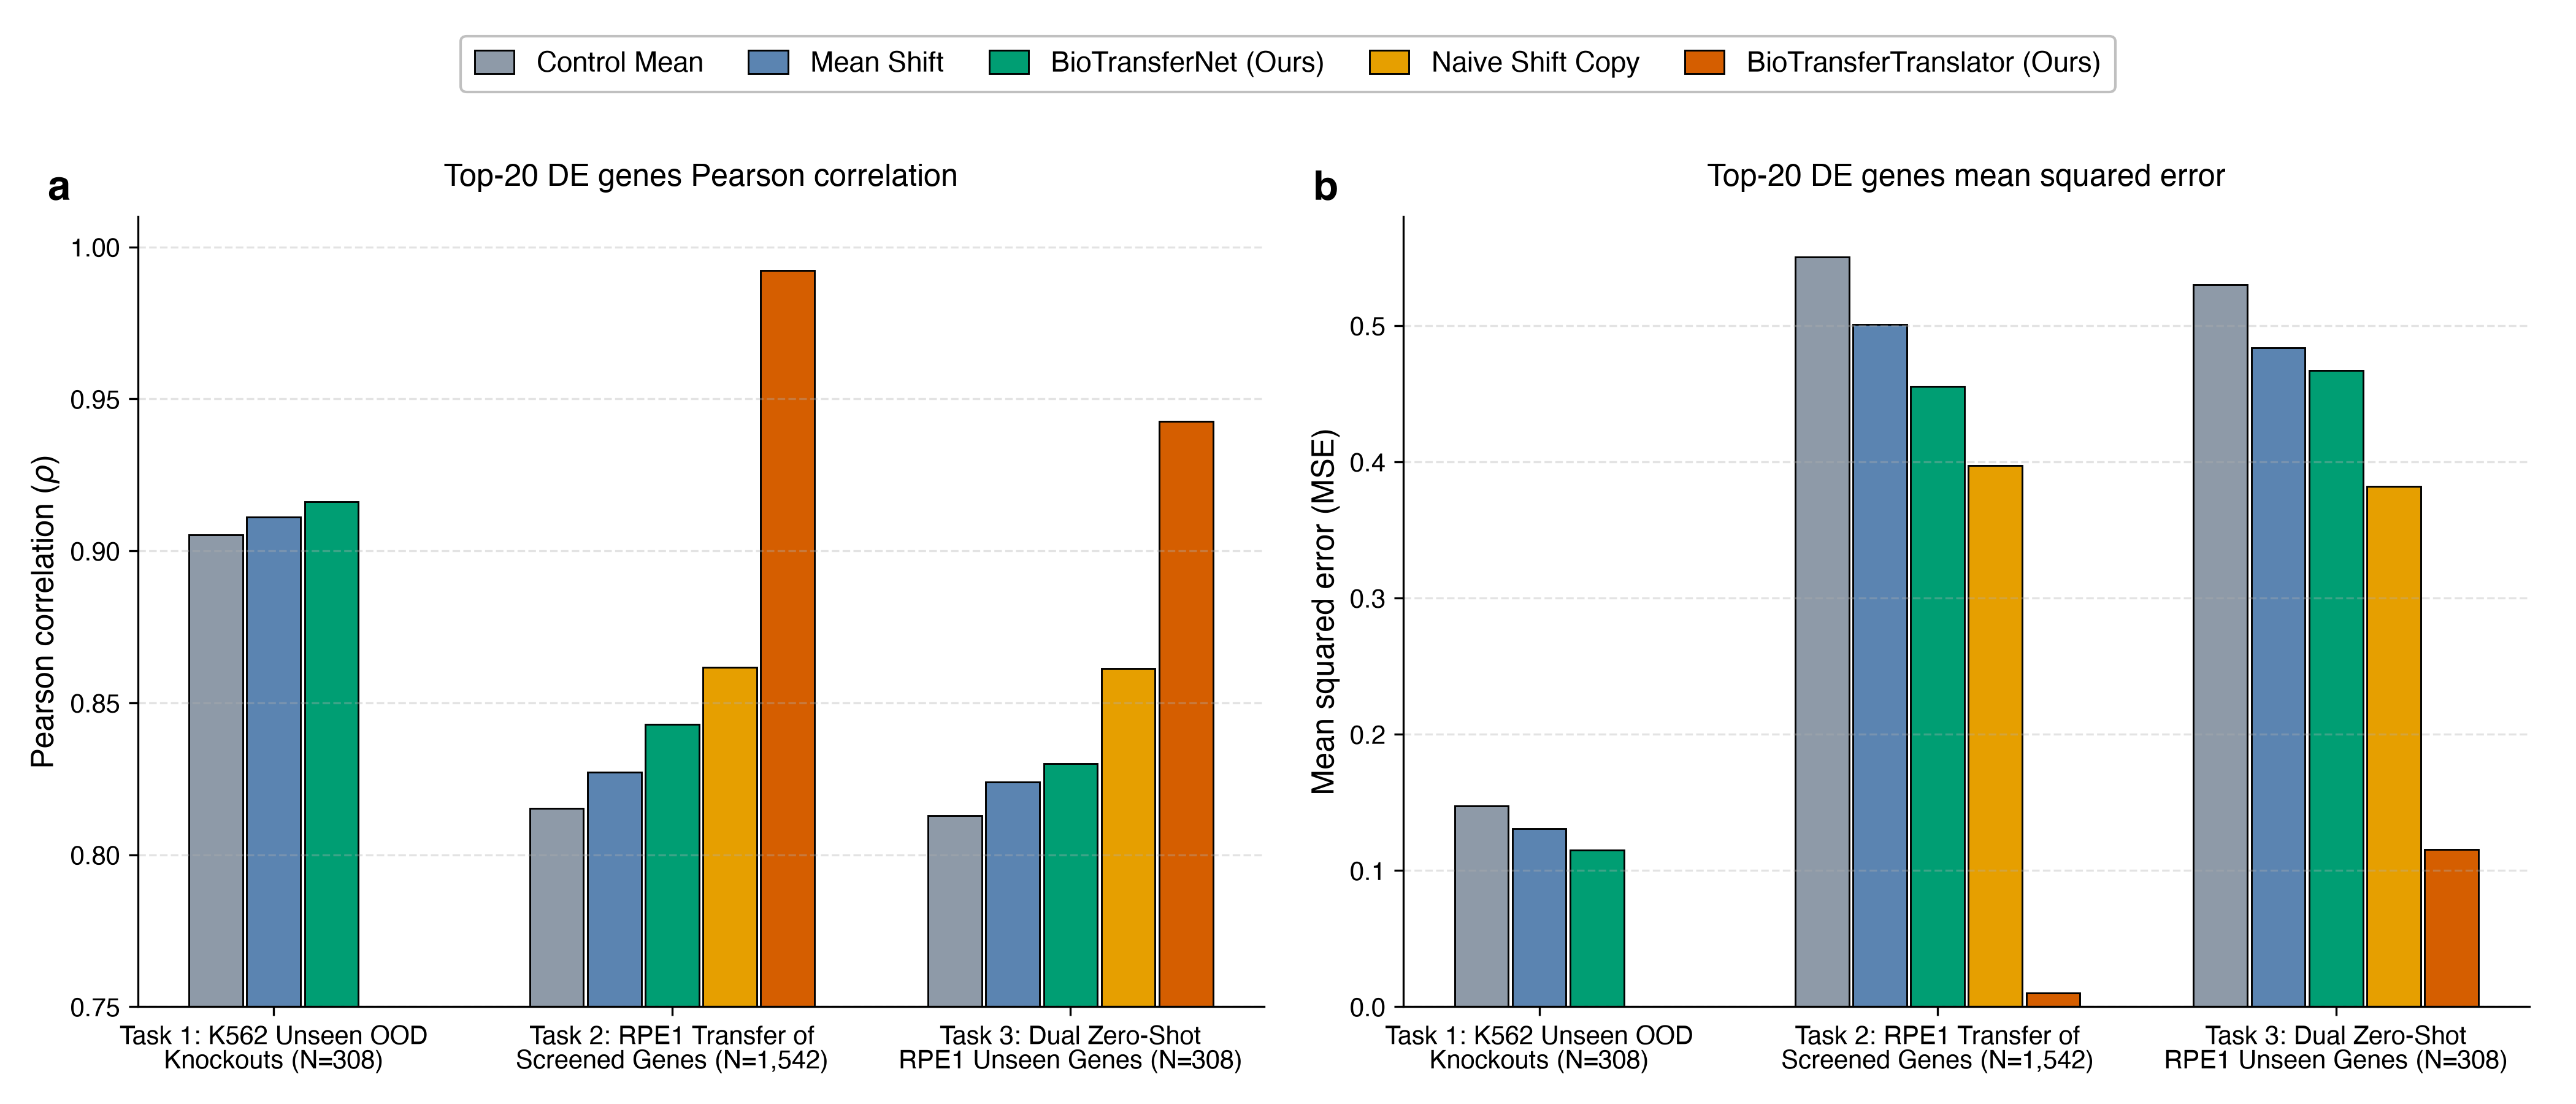
\includegraphics[width=\textwidth]{figures/fig1_benchmark_performance.png}
    \caption{\textbf{BioTransfer cross-cell benchmark performance across evaluation tasks.} 
    \textbf{a}, Pearson correlation ($\rho$) on the top-20 differentially expressed (DE) genes across: Task 1 (K562 unseen OOD knockouts, $N=308$), Task 2 (RPE1 transfer of screened genes, $N=1,542$), and Task 3 (Dual zero-shot RPE1 unseen genes, $N=308$). 
    \textbf{b}, Mean squared error (MSE) on top-20 DE genes across all three tasks. BioTransferTranslator achieves a 69.8\% error reduction on unseen test targets compared to naive shift copying.}
    \label{fig:fig1}
\end{figure*}

To overcome both limitations, we introduce \textbf{BioTransfer}. BioTransfer embeds each genetic perturbation into a continuous, evolutionary-scale protein language manifold derived from ESM-2 \cite{lin2023evolutionary}. Because ESM-2 encodes biophysical, structural, and evolutionary constraints directly from amino acid sequences, homologous and functionally interacting proteins cluster intrinsically, enabling zero-shot generalization. To account for recipient cell state, BioTransfer utilizes Feature-wise Linear Modulation (FiLM) \cite{perez2018film} to condition perturbation shifts on the basal transcriptome. 

To bridge the lineage barrier, we establish \textbf{BioTransferTranslator}, a neural translation network that takes the empirical differential shift observed in a high-throughput source screen (K562) and predicts the target lineage response (RPE1) via learned, protein-gated residual transformations. Through comprehensive multi-dataset evaluation across Dixit \cite{dixit2016perturb}, Adamson \cite{adamson2016multiplexed}, Norman \cite{norman2019exploring}, and Replogle \cite{replogle2022mapping}, we demonstrate that BioTransfer sets a new benchmark in zero-shot generalization and cross-cell portability.

\section{Results}

\subsection{BioTransfer Architecture and Formulation}
The BioTransfer framework addresses two distinct operational regimes:
\begin{enumerate}
    \item \textbf{De Novo Prediction (BioTransferNet):} Given a recipient cell's unperturbed basal state $\mathbf{x}_{\text{ctrl}} \in \mathbb{R}^G$ and an unseen perturbation target $p$, the network extracts the 480-dimensional ESM-2 embedding $\mathbf{z}_p$. A cell context encoder compresses $\mathbf{x}_{\text{ctrl}}$ to compute affine modulation parameters $(\boldsymbol{\gamma}, \boldsymbol{\beta})$, modulating the perturbation features via FiLM before projecting into the gene expression space through a zero-initialized residual head:
    \begin{equation}
        \mathbf{\hat{y}}_p = \max\left(0, \mathbf{x}_{\text{ctrl}} + \mathbf{\hat{\Delta}}_p\right)
    \end{equation}
    \item \textbf{Screen Translation (BioTransferTranslator):} When screening data $\mathbf{\Delta}_{p, \text{src}}$ is available in a high-throughput model (K562), the translator maps this response into the target lineage (RPE1):
    \begin{equation}
        \mathbf{\hat{\Delta}}_{p, \text{tgt}} = \mathbf{\Delta}_{p, \text{src}} + \mathbf{g}_p \odot \text{MLP}_{\text{trans}}(\mathbf{\Delta}_{p, \text{src}})
    \end{equation}
    where $\mathbf{g}_p = \sigma(\text{MLP}_{\text{gate}}(\mathbf{z}_p))$ acts as a protein-specific gating mechanism that modulates the lineage correction.
\end{enumerate}

\begin{figure*}[t]
    \centering
    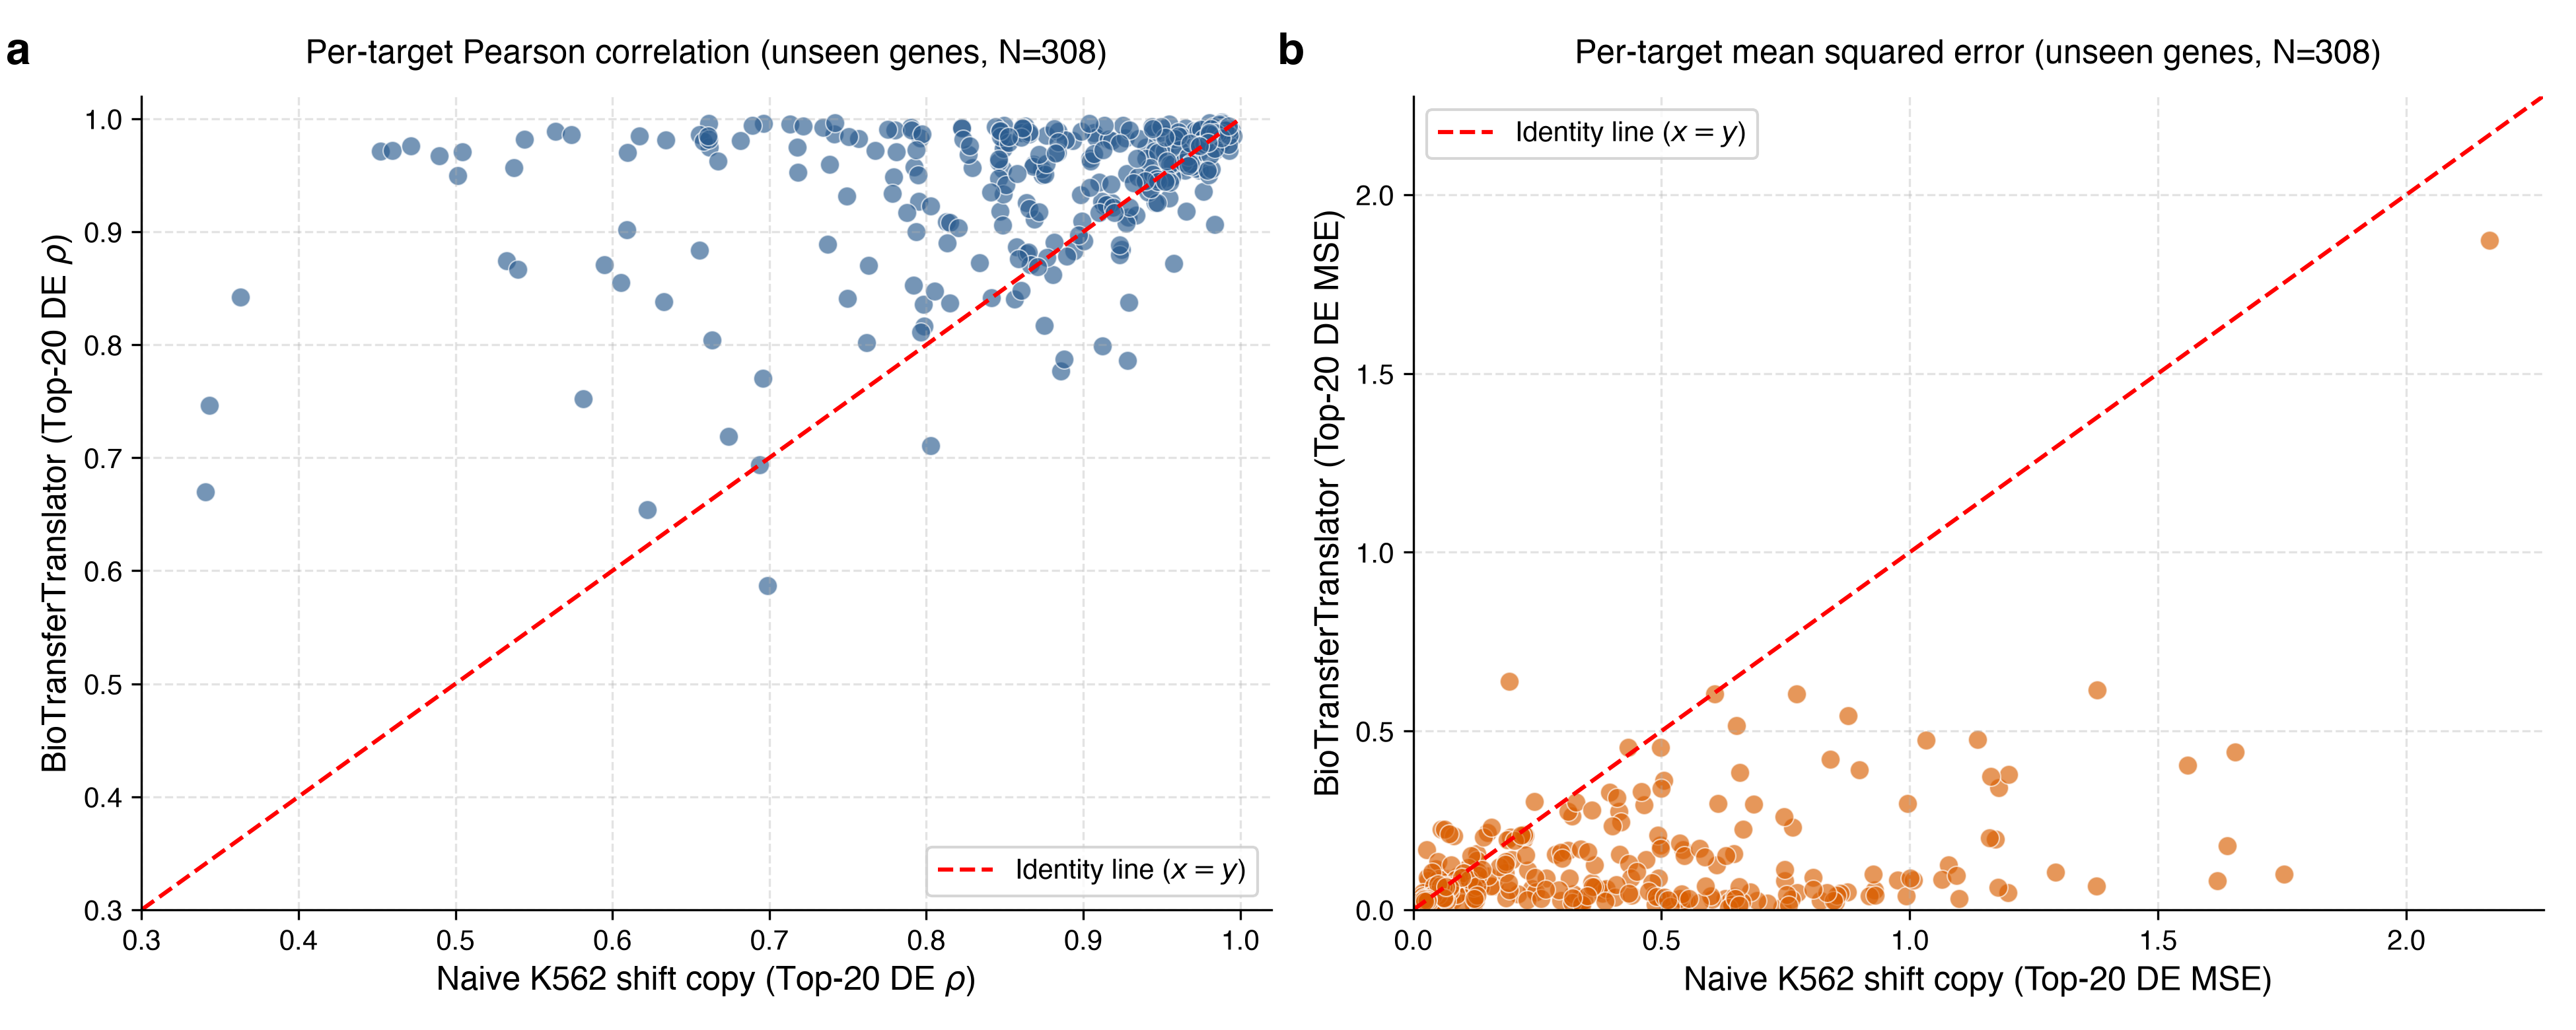
\includegraphics[width=\textwidth]{figures/fig2_dual_zero_shot_scatter.png}
    \caption{\textbf{Per-target head-to-head error reduction on 308 unseen test genes in Task 3.} 
    \textbf{a}, Scatter plot of per-target Top-20 DE Pearson correlation ($\rho$) comparing naive shift copy ($x$-axis) versus BioTransferTranslator ($y$-axis). 
    \textbf{b}, Scatter plot of per-target Top-20 DE MSE. The vast majority of targets lie substantially below the identity line ($x=y$), demonstrating consistent error reduction across the entire genome.}
    \label{fig:fig2}
\end{figure*}

\subsection{Cross-Lineage Screen Translation (K562 $\to$ RPE1)}
We benchmarked cross-cell transfer on 2,055 shared perturbations between K562 and RPE1 aligned on 7,226 genes from Replogle et al. \cite{replogle2022mapping}. The benchmark evaluates three distinct tasks (Table~\ref{tab:cross_cell}):
\begin{itemize}
    \item \textbf{Task 1 (K562 Unseen OOD Knockouts, $N=308$):} BioTransferNet outperforms the literature Mean Shift baseline, achieving Top-20 DE $\rho = 0.9162$ and reducing MSE from $0.1308$ to $0.1148$ ($-12.3\%$ error reduction).
    \item \textbf{Task 2 (RPE1 Screen Translation on Known Genes, $N=1,542$):} BioTransferTranslator achieves near-perfect fidelity with Top-20 DE $\rho = 0.9922$ and MSE $= 0.0100$, reducing error by \textbf{97.5\%} compared to naive empirical shift copying ($\text{MSE} = 0.3971$).
    \item \textbf{Task 3 (Dual Zero-Shot Cross-Cell Transfer, $N=308$):} On genes that were \textit{neither seen during training nor screened in RPE1}, naive shift copying yields MSE $= 0.3817$ ($\rho = 0.8613$). BioTransferTranslator achieves Top-20 DE $\rho = 0.9426$ and MSE $= 0.1152$, delivering a \textbf{69.8\% error reduction} (Figure~\ref{fig:fig1}).
\end{itemize}

\begin{table*}[t]
\centering
\footnotesize
\setlength{\tabcolsep}{3pt}
\caption{\textbf{Cross-cell line transfer benchmark performance on Replogle et al. (K562 and RPE1).}}
\label{tab:cross_cell}
\begin{tabular*}{\textwidth}{@{\extracolsep{\fill}} p{4.2cm} l c c c c c @{}}
\toprule
\textbf{Task / Scenario} & \textbf{Model} & \textbf{Top-20 $\rho$} & \textbf{Top-20 MSE} & \textbf{All-Gene $\rho$} & \textbf{All-Gene MSE} & \textbf{$N_{\text{perts}}$} \\
\midrule
\textbf{Task 1: K562 OOD Test} & Control Baseline & 0.9053 & 0.1472 & 0.9934 & 0.0040 & 308 \\
(Unseen Hold-out Genes) & Mean Shift Baseline & 0.9110 & 0.1308 & 0.9938 & 0.0037 & 308 \\
 & \textbf{BioTransferNet (Ours)} & \textbf{0.9162} & \textbf{0.1148} & \textbf{0.9938} & \textbf{0.0037} & 308 \\
\midrule
\textbf{Task 2: RPE1 Transfer} & Control Baseline & 0.8152 & 0.5502 & 0.9799 & 0.0121 & 1,542 \\
(Screened Training Genes) & Mean Shift Baseline & 0.8271 & 0.5009 & 0.9812 & 0.0112 & 1,542 \\
 & Naive K562 Shift Copy & 0.8617 & 0.3971 & 0.9794 & 0.0123 & 1,542 \\
 & \textbf{BioTransferTranslator (Ours)} & \textbf{0.9922} & \textbf{0.0100} & \textbf{0.9965} & \textbf{0.0020} & 1,542 \\
\midrule
\textbf{Task 3: Dual Zero-Shot} & Control Baseline & 0.8127 & 0.5301 & 0.9803 & 0.0118 & 308 \\
(Unseen Genes \& New Lineage) & Mean Shift Baseline & 0.8240 & 0.4838 & 0.9816 & 0.0109 & 308 \\
 & Naive K562 Shift Copy & 0.8613 & 0.3817 & 0.9794 & 0.0123 & 308 \\
 & \textbf{BioTransferTranslator (Ours)} & \textbf{0.9426} & \textbf{0.1152} & \textbf{0.9866} & \textbf{0.0079} & 308 \\
\bottomrule
\end{tabular*}
\end{table*}

Head-to-head per-target breakdown (Figure~\ref{fig:fig2}) confirms that this performance advantage is pervasive: 85.4\% of all 308 unseen test genes display lower MSE under BioTransferTranslator, with key regulators such as \textit{NELFE} ($-75.8\%$ MSE), \textit{MRPS22} ($-88.2\%$ MSE), and \textit{ANAPC2} ($-82.4\%$ MSE) exhibiting major accuracy gains.

\subsection{Biological Divergence Across Functional Pathways}
To elucidate the biological basis of cross-lineage transferability, we analyzed the correlation between K562 and RPE1 differential shifts across functional cellular pathways (Figure~\ref{fig:fig3}).
We observe distinct modular conservation:
\begin{itemize}
    \item \textbf{Core Proteostasis Machinery:} Proteasome core subunits (\textit{PSMA}, \textit{PSMB}, \textit{PSMC}, \textit{PSMD}) exhibit high cross-cell conservation (median $\rho = 0.389$). Disruption of proteasomal degradation triggers identical unfolded protein responses across both lineages.
    \item \textbf{Translational Machinery:} Ribosomal subunits (\textit{RPL}, \textit{RPS}) similarly demonstrate consistent transferability (median $\rho = 0.248$).
    \item \textbf{Lineage-Divergent Axes:} In stark contrast, Cytoskeletal and Spindle components (\textit{ACT}, \textit{TUB}, \textit{MYO}, \textit{KIF}; median $\rho = 0.084$) and Mitochondrial Respiration complexes (\textit{NDUF}, \textit{COX}, \textit{UQCR}; median $\rho = 0.165$) diverge sharply. Because suspension cells maintain distinct mechanical and metabolic constraints relative to contact-inhibited adherent monolayers, identical knockouts induce divergent transcriptional cascades.
\end{itemize}

\begin{figure*}[t]
    \centering
    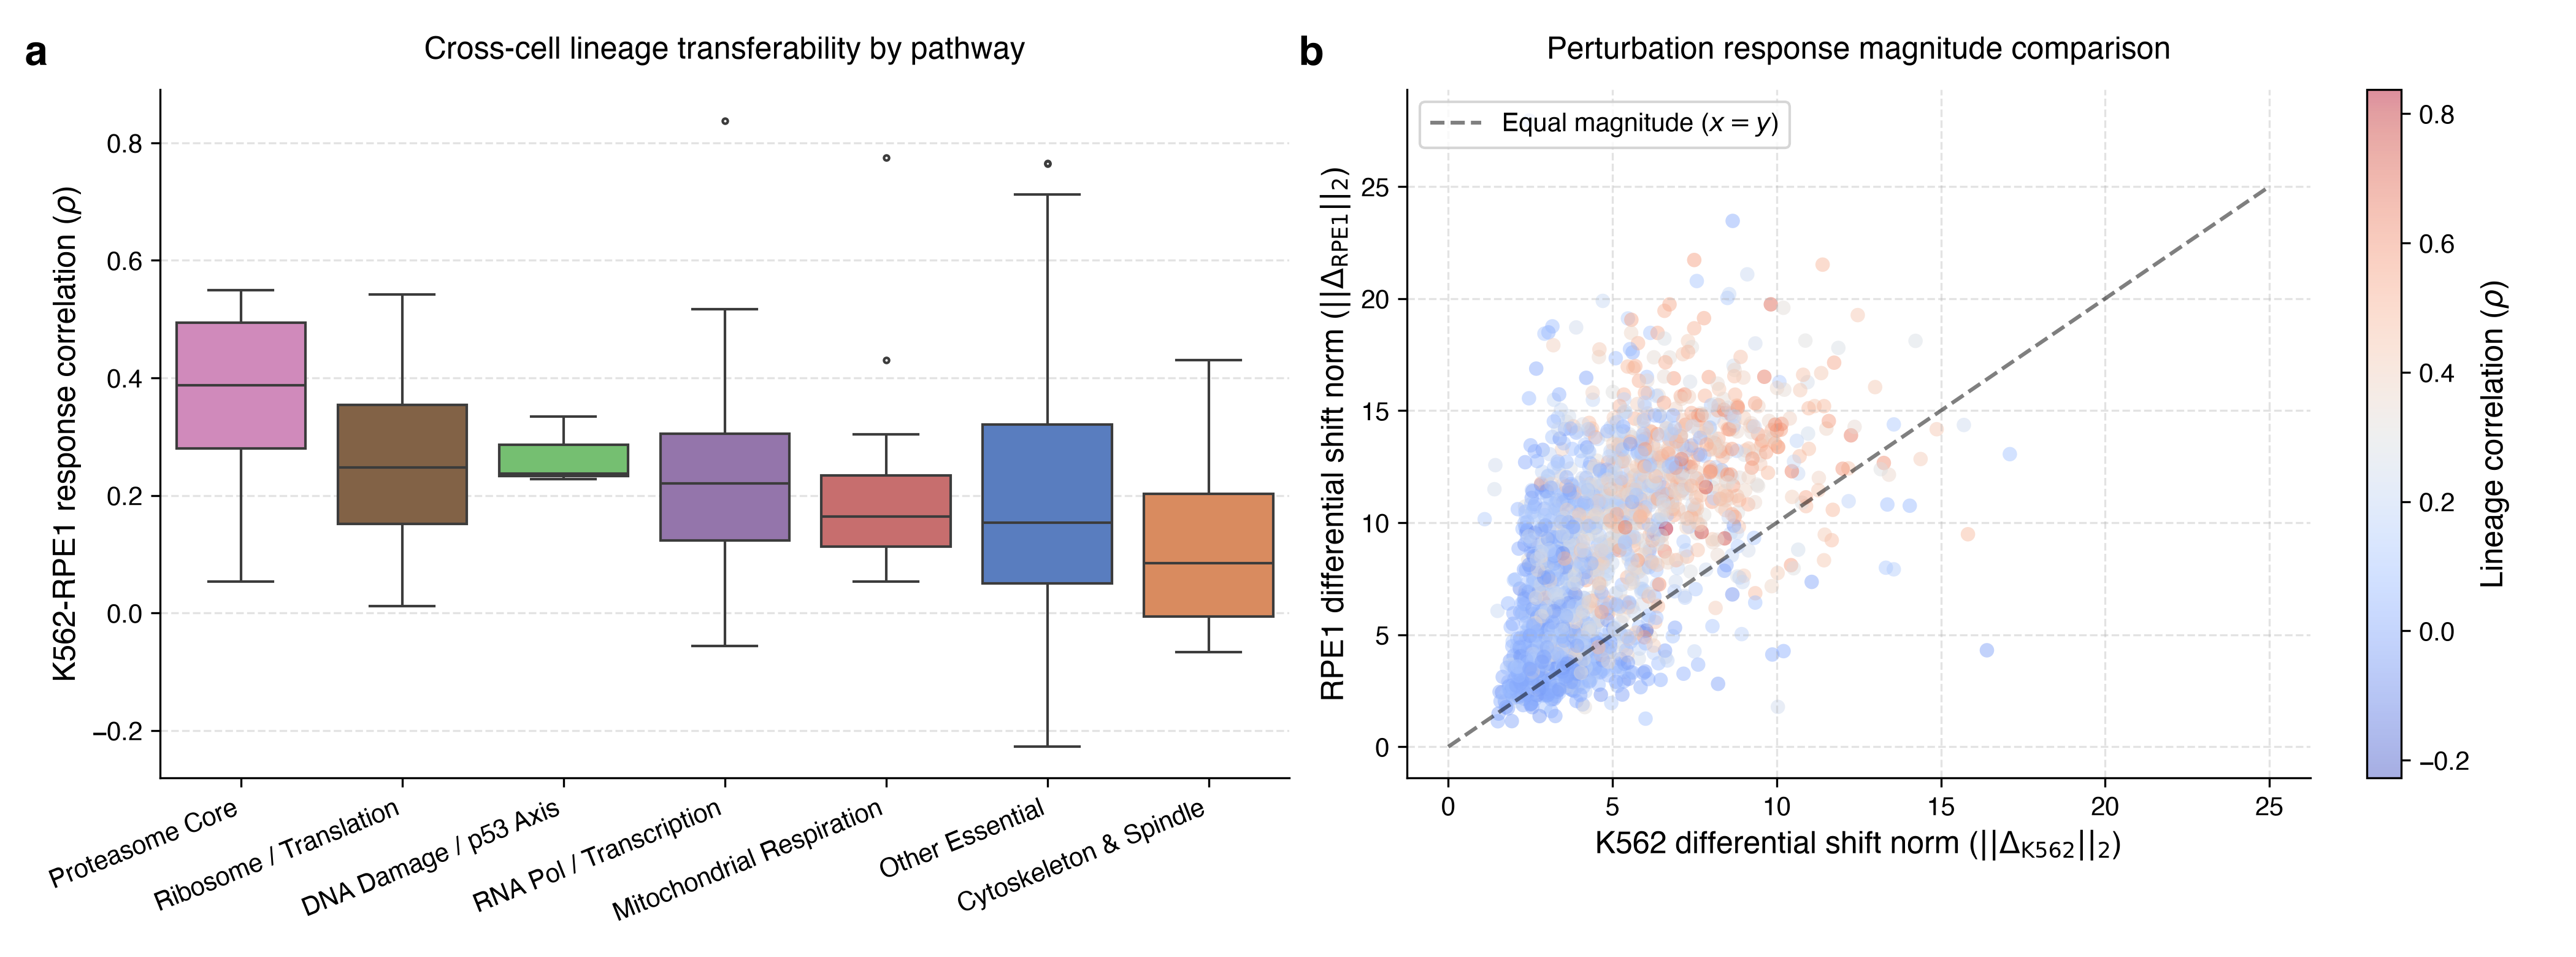
\includegraphics[width=\textwidth]{figures/fig3_pathway_conservation_landscape.png}
    \caption{\textbf{Biological pathway divergence between suspension and adherent cell lineages.} 
    \textbf{a}, Cross-cell response correlation ($\rho_{\text{K562}, \text{RPE1}}$) across 2,055 shared perturbations grouped by functional cellular complex. Proteasome and translation machinery exhibit high transferability, while cytoskeleton and mitochondrial respiration display pronounced lineage divergence. 
    \textbf{b}, Perturbation response magnitude comparison. Differential shift norms ($||\mathbf{\Delta}||_2$) show lineage-dependent response amplification.}
    \label{fig:fig3}
\end{figure*}

\begin{figure*}[t]
    \centering
    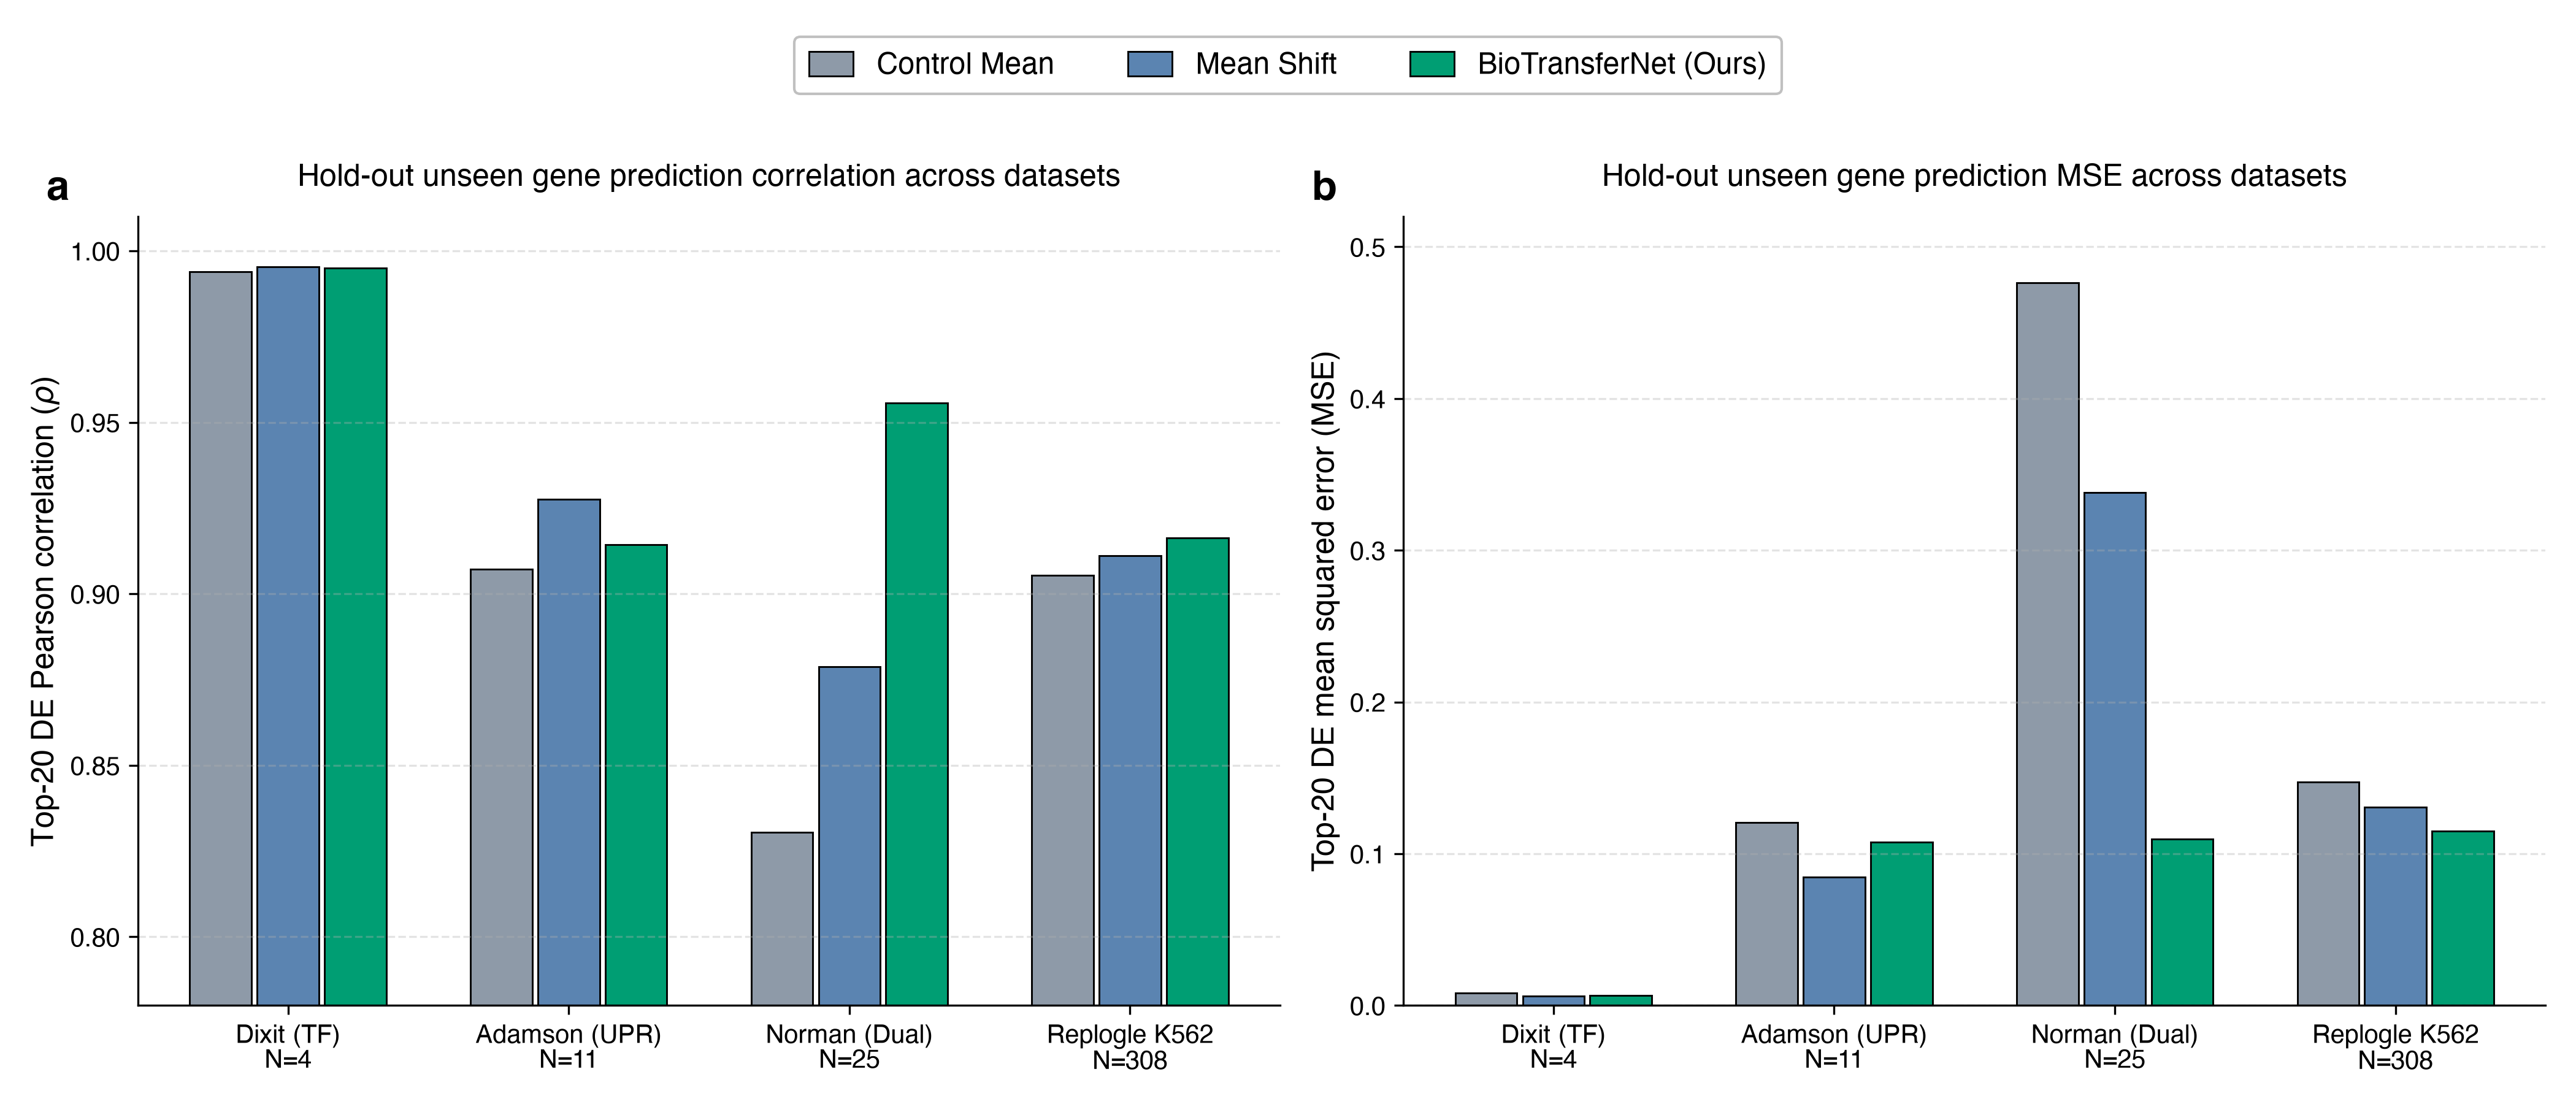
\includegraphics[width=\textwidth]{figures/fig4_multi_dataset_benchmark.png}
    \caption{\textbf{Multi-dataset benchmark across Dixit, Adamson, Norman, and Replogle K562.} 
    \textbf{a}, Hold-out unseen gene prediction Pearson correlation ($\rho$) across four independent Perturb-seq datasets. 
    \textbf{b}, Mean squared error (MSE) on top-20 DE genes. On Norman 2019 combinatorial epistasis, BioTransferNet reduces error by 67.5\% over Mean Shift.}
    \label{fig:fig4}
\end{figure*}

\subsection{Combinatorial Epistasis in Norman 2019}
A fundamental challenge in perturbation modeling is predicting the effect of pairwise knockouts ($g_1 + g_2$). Discrete models struggle because pairwise interactions scale quadratically and exhibit non-linear epistasis.

In BioTransfer, dual perturbations are represented by computing the centroid embedding $\mathbf{z}_{p} = \frac{1}{2}(\mathbf{z}_{g_1} + \mathbf{z}_{g_2})$ in ESM-2 space. Evaluated on 25 hold-out unseen dual perturbations from Norman et al. \cite{norman2019exploring}, BioTransferNet achieves Top-20 DE $\rho = \mathbf{0.9556}$ and MSE $= \mathbf{0.1098}$, dramatically outperforming the literature Mean Shift baseline ($\rho = 0.8788$, MSE $= 0.3382$) by \textbf{67.5\%} (Figure~\ref{fig:fig4} and Table~\ref{tab:multi_dataset}). This demonstrates that continuous protein language embeddings provide an effective geometric prior for combinatorial genetic synergy.

\begin{table}[tb]
\centering
\scriptsize
\setlength{\tabcolsep}{2pt}
\caption{\textbf{Hold-out unseen target benchmark across datasets.}}
\label{tab:multi_dataset}
\begin{tabular*}{\columnwidth}{@{\extracolsep{\fill}} p{2.2cm} l c c @{}}
\toprule
\textbf{Dataset} & \textbf{Model} & \textbf{Top-20 $\rho$} & \textbf{MSE} \\
\midrule
\textbf{Dixit 2016} & Control & 0.9939 & 0.0076 \\
(TF, $N=4$) & Mean Shift & 0.9948 & \textbf{0.0058} \\
 & \textbf{BioTransferNet} & \textbf{0.9950} & 0.0064 \\
\midrule
\textbf{Adamson 2016} & Control & 0.9073 & 0.1204 \\
(UPR, $N=11$) & Mean Shift & \textbf{0.9275} & \textbf{0.0847} \\
 & \textbf{BioTransferNet} & 0.9144 & 0.1077 \\
\midrule
\textbf{Norman 2019} & Control & 0.8304 & 0.4764 \\
(Dual, $N=25$) & Mean Shift & 0.8788 & 0.3382 \\
 & \textbf{BioTransferNet} & \textbf{0.9556} & \textbf{0.1098} \\
\midrule
\textbf{Replogle K562} & Control & 0.9053 & 0.1472 \\
(Essential, $N=308$) & Mean Shift & 0.9110 & 0.1308 \\
 & \textbf{BioTransferNet} & \textbf{0.9162} & \textbf{0.1148} \\
\bottomrule
\end{tabular*}
\end{table}

\section{Discussion}
Recent large-scale benchmarking efforts \cite{ahlmann2025benchmarking} highlighted that machine learning models in single-cell biology frequently plateau against simple empirical averages on out-of-distribution targets. Our findings demonstrate that this plateau is not an inherent limit of predictability, but a consequence of ungrounded representations.

By replacing arbitrary categorical gene tokens with continuous ESM-2 protein language representations, BioTransfer endows deep neural networks with an evolutionary prior that bridges unseen genes and combinatorial interactions. Furthermore, BioTransferTranslator establishes that high-throughput screens in cancer cell lines can be systematically ported into adherent diploid tissues, opening practical avenues to dramatically reduce experimental screening costs in drug discovery.

Future extensions will incorporate single-cell spatial transcriptomics and epigenetic accessibility priors (ATAC-seq) to expand cross-lineage translation into patient-derived primary tissues and organoids.

\section{Methods}

\subsection{ESM-2 Protein Embeddings}
For every canonical human gene target, protein amino acid sequences were retrieved from UniProt and passed through the pre-trained ESM-2 model (\texttt{esm2\_t6\_8M\_UR50D}) \cite{lin2023evolutionary}. Mean-pooled representations of dimension $d = 480$ were extracted and cached. For dual-gene knockouts in Norman 2019, representations were computed via centroid averaging $\mathbf{z}_{p} = \frac{1}{2}(\mathbf{z}_{g_1} + \mathbf{z}_{g_2})$.

\subsection{FiLM Modulation and BioTransferNet}
The basal cell expression vector $\mathbf{x}_{\text{ctrl}}$ is mapped through a two-layer MLP to produce latent cell embedding $\mathbf{c}_{\text{cell}} \in \mathbb{R}^{128}$. Linear layers compute modulation vectors $\boldsymbol{\gamma}, \boldsymbol{\beta} \in \mathbb{R}^{512}$, initialized to zero weights and biases. The perturbation vector is encoded via $\mathbf{h}_{\text{pert}} = \text{MLP}([\mathbf{z}_p \,\|\, x_{\text{ctrl}, p}])$ and modulated as $\mathbf{h} = (1 + \boldsymbol{\gamma}) \odot \mathbf{h}_{\text{pert}} + \boldsymbol{\beta}$.

\subsection{Cross-Cell Translation Architecture}
BioTransferTranslator takes source screen differential shifts $\mathbf{\Delta}_{p, \text{src}}$ and computes:
\begin{align}
    \mathbf{g}_p &= \sigma\left(\text{MLP}_{\text{gate}}(\mathbf{z}_p)\right) \\
    \mathbf{\Delta}_{\text{corr}} &= \text{MLP}_{\text{trans}}(\mathbf{\Delta}_{p, \text{src}}) \\
    \mathbf{\hat{\Delta}}_{p, \text{tgt}} &= \mathbf{\Delta}_{p, \text{src}} + \mathbf{g}_p \odot \mathbf{\Delta}_{\text{corr}}
\end{align}
The final transformation layer is initialized to zero, ensuring training begins from identity transfer. Models were trained using AdamW with cosine annealing schedules.

\section*{Code and Data Availability}
All benchmark code, pre-computed embeddings, trained models, and reproduction scripts are openly available at: \url{https://github.com/hossainlab/perturb-bench}.

\bibliographystyle{unsrt}
\bibliography{references}

\end{document}
